\documentclass[a4paper]{book}

\usepackage{fullpage} % Package to use full page
\usepackage{parskip} % Package to tweak paragraph skipping
\usepackage{tikz} % Package for drawing

\usepackage{hyperref}
\usepackage{amsmath}
\usepackage{amssymb}
\usepackage{amsthm}
\usepackage{enumitem}

\newtheorem{theorem}{Theorem}%[section]
\newtheorem{corollary}{Corollary}%[theorem]
\usepackage{subcaption}

\title{Coloring of Planar Graphs}
\author{}
\date{}
\date{\vspace{-5ex}}

\begin{document}

\maketitle

\section*{Four-color Problem}
For any planar graph $G,\chi(G)\leq 4$.\\
e.g.: $K_4-planar$
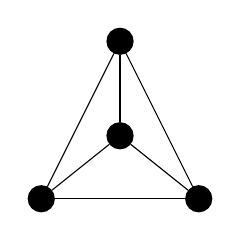
\begin{tikzpicture}[auto]
    \begin{scope}[every node/.style={circle,fill, draw=black,minimum size=1mm}]
        \node (A) at (0,1) {};
        \node (B) at (1,-1) {};
        \node (C) at (-1,-1) {};
        \node (D) at (0,-0.2) {};
    \end{scope}
    \begin{scope}[every edge/.style={draw=black}]
        \draw (A) edge node{} (B);
        \draw (A) edge node{} (C);
        \draw (A) edge node{} (D);
        \draw (B) edge node{} (C);
        \draw (B) edge node{} (D);
        \draw (C) edge node{} (D);
    \end{scope}
\end{tikzpicture}
\section*{Five-color Theorem}
\begin{theorem}
Every planar graph is 5-colorable.
\end{theorem}
\begin{proof} By contradiction.\\\\
Assume that $\exists$ some planar graphs that are impossible to color with 5 colors.\\
Let $G=(V,E)$ be such graphs with minimum $|V|$ that cannot be colored with five colors.\\\\
From the corollary of Euler's theorem $e\leq 3v-6\Rightarrow\sum_{u\in V}deg(u)=2e\leq6v-12<6v$.\\ Thus, by Pigeon hole Principle, $\exists$ vertex $x\in V, deg(x)<\frac{6v}{v}=6$. So, $deg(x)\leq5$. Consider $H=G-x$ (by remoing $x$ and its incident edges). By our assumption, graph $H$ is 5-colorable. Assume that $x$ was adjacent (in $G$) to the vertices $x_1,x_2,\cdots,x_k (k\leq5)$.\\
If at most 4 colors are used to color vertices $x_1,x_2,\cdots,x_k$ in a 5-coloring of graph $H$, then $x$ can be colored with one of the remaining colors. Thus $G$ will be 5-colorable, contradiction. So, $k=5, deg(x)=5$ and all vertices $x_1,x_2,\cdots,x_5$ have different colors in a 5-coloring of graph $H$.\\
(5 color but disconnected)Denote by $H(i,j)$ the subgraph of $H$ spanned by vertices of color $i$ and $j$. Assume that $x_1,x_2,\cdots,x_5$ are in cyclic order about $x$, and the color of $x_i$ is $i,i=1,2,\cdots,5$. If $x_i$ and $x_j$ belong to distinct connected components of $H(i,j)$, then by interchanging the colors $i$ and $j$ in the component of $x_j$ we obtain another coloring of $H$ where both $x_i$ and $x_j$ get colors $i$. So, color $j$ is not used to color any of the vertices $x_1,x_2,\cdots,x_5$. Then, color $x$ by $j$, contradiction, $G$ was not 5-colorable.\\
Suppose $x_i$ and $x_j$ belong to the same connected componet of $H(i,j),\exists$ $x_1$~$x_5$ path $P_{ij}$ in $H$ whose vertices are colored $i$ and $j$. Similarly, $H$ must contain an $x_2$~$x_4$ path $P_{24}$ whose vertices are colored $2$ and $4$ (if no, interchanging color 2 and  4 in the componet of $x_2$ within $H(2,4)$ we arrive to contradiction as before). However, this is impossible, since circuit $x_1P_{13}x_3$ of $G$ seperates $x_2$ from $X4$, and path $P_{24}$ cannot intersect this circuit (since $G$ is planar).
\end{proof}
\end{document}